\documentclass[a4paper,oneside,12pt]{article}
\usepackage{ctex}
\usepackage{graphicx}
\usepackage{geometry}
\geometry{left = 2.5cm, right = 2.5cm, top = 2cm, bottom = 2cm}

\newcommand{\bol}[1]{\textbf{#1}}
\newcommand{\diff}{\mathrm{d}}

\title{刘维烨专用资料}
\author{Xiaoyu Xue}
\date{\today}

\begin{document}
\maketitle
\section{数学}
\subsection{数学符号}
\begin{enumerate}
	\item 求和: $\displaystyle \sum_{i = 0} ^ n a_i = a_0 + \ldots + a_n$
	\item 坐标: 三维坐标用$(x,y,z)$表示
	\item 向量: $\vec{a}$或者$\bol{a}$,三维向量$\bol{a} = (x,y,z)$
	\item 有限元差分: 用$\Delta x$来表示两个物理量$x1,~x2$的变化量
\end{enumerate}
\subsection{向量}
\subsubsection{向量的长度}
$\bol{a} = (x_1, y_1, z_1)$,向量$\bol{a}$的长度为
\begin{displaymath}
\vert \bol{a} \vert = \sqrt{x_1^2 + y_1^2 + z_1^2}
\end{displaymath}
\subsubsection{向量加法}
$\bol{a} = (x_1, y_1, z_1)$,$\bol{b} = (x_2, y_2, z_2)$,三角形或者平行四边形准则
\begin{displaymath}
\bol{a} + \bol{b} = (x_1 + x_2, y_1 + y_2, z_1 + z_2)
\end{displaymath}
\vspace{-10mm}
\begin{figure}
\centering
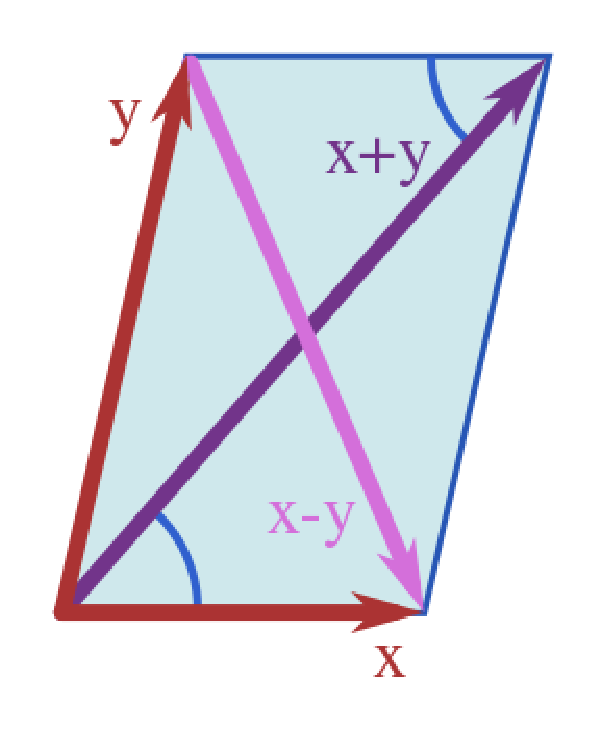
\includegraphics[scale=0.4]{./figure/fig1.eps}
\end{figure}
\subsubsection{向量数乘}
一个数乘一个向量的结果是一个向量
\begin{displaymath}
c\bol{a} = c(x, y, z) = (cx, cy, cz)
\end{displaymath}
\subsubsection{向量点乘}
向量点乘的结果是一个标量:
\begin{displaymath}
\bol{a} \cdot \bol{b} = \vert \bol{a}\vert \vert\bol{b}\vert \cos\theta =x_1x_2 + y_1y_2 + z_1z_2
\end{displaymath}
\subsubsection{向量叉乘}
向量叉乘的结果是一个向量,长度为
\begin{displaymath}
\vert\bol{a}\times\bol{b}\vert = \vert\bol{a}\vert \vert\bol{b}\vert \sin\theta
\end{displaymath}
\par 向量为:
\begin{displaymath}
\bol{a}\times\bol{b} = \left\vert
\begin{array}{ccc}
\bol{i} & \bol{j} & \bol{k}\\
x_1 & y_1 & z_1\\
x_2 & y_2 & z_2
\end{array}
\right\vert = \left(y_1z_2 - y_2z_1 , x_2z_1 - x_1z_2 , x_1y_2  - x_2y_1\right)
\end{displaymath}
\par 向量的方向根据坐标系选择左右手法则(不满足交换律)
\begin{figure}[!h]
\centering
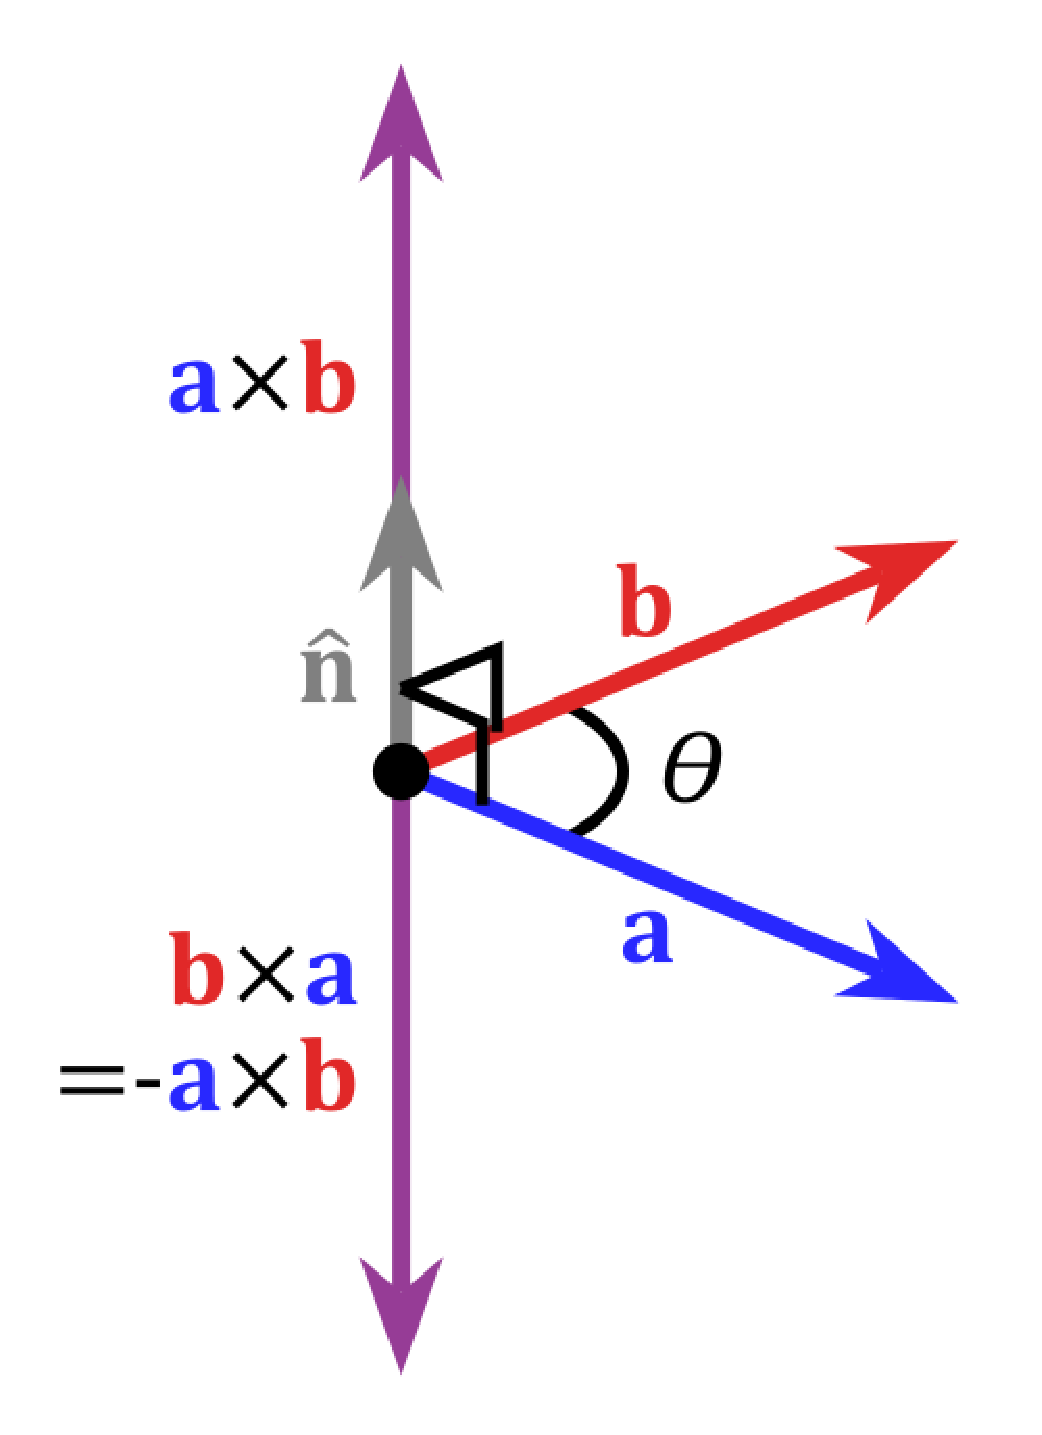
\includegraphics[scale=0.3]{./figure/fig2.eps}
\end{figure}

\section{位移、速度和加速度}
\subsection{位移}
定义:由初位置到末位置的一段有向线段(向量)\\
假设点A的位置为$\bol{a} = (x_1, y_1, z_1)$,点B的位置为$\bol{b} = (x_2, y_2, z_2)$,A到B的位移为$\bol{x} = \bol{b} - \bol{a} = (x_2 - x_1 , y_2 - y_1, z_2 - z_1)$
\subsection{速度}
定义:一个物体的速度定义成在某个参考系下它的位置的变换率,是一个随时间变化的函数,可以用$\bol{v}(t)$表示
\subsubsection{平均速度(Average velocity)}
\begin{displaymath}
	\bar{\bol{v}} = \frac{\Delta \bol{x}}{\Delta t}
\end{displaymath}
其中$\Delta \bol{x}$表示位移,$\Delta t$表示经历的时间
\subsubsection{瞬时速度(Instantaneous velocity)}
\begin{displaymath}
	\bol{v} = \lim_{\Delta t \to 0}\frac{\Delta \bol{x}}{\Delta t} = \frac{\diff\bol{x}}{\diff t}
\end{displaymath}
因此位移可以通过瞬时速度的积分求得
\begin{displaymath}
\bol{x} = \int\bol{v}\diff t
\end{displaymath}
\subsection{加速度}
定义:加速度为速度随时间的变化率(向量),是一个时间的函数,用$\bol{a}(t)$表示
\subsubsection{平均加速度(Average acceleration)}
\begin{displaymath}
	\bar{\bol{a}} = \frac{\Delta \bol{v}}{\Delta t}
\end{displaymath}
其中$\Delta \bol{v}$为速度差,$\Delta t$为经历的时间
\subsubsection{瞬时加速度(Instantaneous acceleration)}
\begin{displaymath}
	\bol{a} = \lim_{\Delta t \to 0} \frac{\Delta \bol{v}}{\Delta t} = \frac{\diff \bol{v}}{\diff t}
\end{displaymath}
可以看出瞬时加速度是速度随时间的导数,速度优势位移随时间的导数,所以加速度是位移随时间的二阶导数
\begin{displaymath}
	\bol{a} = \frac{\diff \bol{v}}{\diff t} = \frac{\diff^2 \bol{x}}{\diff t^2}
\end{displaymath}
\section{受力分析}
\section{牛顿运动定律}
\section{圆周运动}
\end{document}